\documentclass[12pt,twocolumn]{article}
\usepackage[margin=1.0in]{geometry}

\usepackage{graphicx}
\usepackage[font=footnotesize,labelfont=bf]{caption}

\usepackage{hyperref}

\usepackage[backend=biber]{biblatex}
\usepackage[british]{babel}
\addbibresource{report.bib}
\author{
    Mohamed Ibrahim Atallah 
    \\
    Prof. Dr. Ayman Abdel-Hamid
    \\
    \\ 
    College of Computing and Information Technology 
    \\ 
    Arab Academy for Science, Technology and Maritime Transport}
\title{Peer-to-Peer Security}
\begin{document}
\maketitle
\begin{abstract}
    Developments to peer-to-peer systems have been revolutionary in many ways, 
    Napster, Gnutella and BitTorrent were some of the first P2P application that
    gave the world a glimpse of their true potential, later with the inception of
    distributed ledger by Bitcoin, that brought a way to solve the double spending
    problem. P2P also brought a way to combat censorship and provide anonymization
    services to those who need it via Tor. This report attempts to survey
    the security implications of P2P.
\end{abstract}

\section{Introduction}
Peer-to-Peer (P2P) systems present a unique set of security challenges, while some of
these challenges are new and unique to P2P systems, most of them are in fact the same 
security challenges we're already aware of but amplified due to the inherent complexity of P2P.
In the traditional client-server systems we always had a central
authority to trust. To this end, the target of any potential attack is the server and
any disputes in the system are resolved by the server as well, and so we had a single 
point of both trust and failure. On the other hand in P2P systems, peers have mostly 
similar roles they can be clients or servers an early example of this is BitTorrent 
\cite{bittorrent}, where peers can be clients (i.e., downloaders, \emph{leechers}), 
servers (i.e., uploaders, \emph{seeders}), or simultaneously uploading pieces of files they
have and downloading pieces of files they don't have. Effectively being both the client and 
the server at the same time. We can quickly see the attractiveness of this model, the burden of
sharing files is no longer carried out by some central resource but shared among peers 
to achieve a common goal.


The emergence of blockchain and cryptocurrencies initiated by Bitcoin \cite{bitcoin}, 
sparked major interest in P2P systems, with major companies touting what is so called ``The Metaverse'' 
to be the future, governed by blockchain technologies. However, before that dystopian nightmare
becomes a reality we need to
understand its security implications.

Contributions of this report are the following: we explore these security challenges 
in the domain of P2P systems, major innovations and how it addresses these challenges 
we also provide an in-depth review of recent works in P2P security regarding 
the following topics:
\begin{itemize}
    \item Peer Discovery 
    \item Message Propagation
    \item Consensus
\end{itemize}

\section{Background}
This section presents the conceptual framework, on which we will base our understanding
of P2P systems. Let us begin with a formal definition of what is a P2P system derived from
the ideas we discussed so far. A P2P system is a system in which peers have symmetric functions,
where how performant the system is determined by the peers and their shared resources, rather than
a central resource, and so a single word can describe such system \textbf{decentralization}. 
Now we can categorize P2P systems as such \cite{ds:book}:
\begin{itemize}
    \item Structured: peers are organized in a deterministic topology (rings, binary trees, grids, etc.)
    \item Unstructured: peers maintain an ad-hoc list of neighbors
\end{itemize}

\subsection{Peer Discovery}
Secure peer discovery is the process of finding identifiers of other nodes (peers) in the network, 
while maintaining the following invariants \cite{guarded_gossip}:
\begin{enumerate}
    \item Peer discovery is unbiased (a form of active attacks)
    \item Avoiding information leakage (a form of passive attacks)
\end{enumerate}


\subsubsection{Centralized Discovery}
One solution to our discovery task is to utilize a central directory authority (including replicas) \cite{bittorrent, tor:directory_spec}
that keeps track of all active peers in the network, whenever a new node joins the network it registers itself with that authority,
and gets a list of nodes to establish connections. However, this approach is flawed in many aspects: first, 
it proposes a trust bottleneck as observed in Tor \cite{tor:directory_spec}
if a single directory authority lied, it could make clients believe for a time a distorted view of the network,
second, a scaling bottleneck as directory require tracking of more peers with a high rate of node churn,
third, it presents a target for attacks on the system \cite{tor:censor, egypt:censor}
\begin{figure}[h]
    \includegraphics[width=\linewidth]{fig/p2p_report.png}
    \caption{Centralized solution showing nodes different connections achieved by using a Directory Authority (DA)}
\end{figure}

\subsubsection{Structured P2P Discovery: DHT \label{DHT}}
Distributed hash table (DHT) is purely P2P solution, that doesn't rely on a central resource for discovery.
Chord \cite{chord} is one of the prominent DHT systems used for discovery, where every node gets assigned a \textbf{key},
produced from applying a cryptographic hash function to a unique node identifier (e.g., IP Address). Peers in the system 
should not be able to influence the key they get assigned (the result of the hash function), and other peers in the system
should easily verify the authenticity of the assigned key through applying the same hash function. 


Peers then keep track of their immediate successor (first node with a higher key value) and predecessor
and a finger table (FT), each finger entry consist of a starting key value and the immediate successor node of that key,
FT provide convenient shortcuts to resolve key lookups. In fact, Chord key lookup has worst case complexity of 
$\mathcal{O}(\log n)$ \cite{chord} where $n$ is the number of nodes,
if the lookup key doesn't exist in our best guess finger node we know of from our FT, that node would forward our key lookup request to
best finger node it knows of from its FT, and so on, and so forth until the lookup is resolved. However, this method of looking up a key has one major
drawback is that it violates one of our node discovery invariants. Here information leakage occurs, intermediate nodes are aware of our lookup target.

A suggested solution to this problem would be request the FT of other peer instead of sending them our lookup target. 
This approach is still vulnerable to both passive and active attacks:
\begin{enumerate}
    \item A malicious node may manipulate their own FT by 
        omitting honest nodes in favour of colluding malicious nodes.
    \item Information leakage may still occur if the fraction of malicious node is 
        high enough such that malicious nodes can utilize the Chord structure 
        to deduce information about our lookup target.
\end{enumerate}
\begin{figure}[h]
    \includegraphics[width=\linewidth]{fig/peer_discovery_dht.png}
    \caption{Chord key lookup}
\end{figure}

\subsection{Blockchain\label{Blockchain}}
A widespread (and notorious \cite{crypto:ban}) application of P2P is blockchain
and first of which was Bitcoin \cite{bitcoin}. Interactions between peers on a blockchain
is expressed through transactions. A transaction is message between two parties $X$ and $Y$ that includes the digital signature \cite{security_book} of $X$
and the hash of the previous transaction forming a \textit{chain} that latest of which transfers the ownership of some digital asset to $Y$. 
The problem remains how can $Y$ verify that $X$ didn't double spend that digital asset in an earlier transaction?
In absence of a central authority the solution is to publicly announce transactions to the network. Now only the earliest transaction is the one that
counts and later transactions are deemed invalid.

We need some sort of system to come to an agreement on the truth of the chronological order of transactions,
with the lack of trust in P2P environment makes this a truly challenging task as all peers can be potential attackers.

We also need a way to commit transactions to the network, associating them to a specific timestamp, in order to prevent replay attacks. 

Blocks are a collection of verified transactions and acts a form of commit of transactions to the networks, that is, when a transaction is added
to a block it cannot be modified or reverted, since blocks also contain a hash of
the previous block forming a \textit{chain}, and thus the name, blocks should preserve the chronological order of transactions.


\subsubsection{Nakamoto Consensus}
The breakthrough of Bitcoin was its consensus mechanisms, Proof-of-work (PoW) and the longest chain rule together form agreement among untrustworthy peers.
Although the idea of PoW wasn't a new as it was first introduced as a mean to protect against spam e-mails\cite{pow:origin}, 
it was the first of its kind to be employed in a P2P environment to reach consensus. 


PoW constitutes that peers work on ``mining'' blocks by collecting and verifying transactions into a block and then work on generating a new hash
for that block by changing a nonce value to get a hash that starts with a certain number of consecutive $0$ bits determined by a 
\textit{mining difficulty} parameter, determined by the number of miners active on the network.
Once that nonce value is found, the block is now considered \textit{mined} and the miner then broadcasts that block
to the network and peers can then easily verify that block, and move on to mining the next block.

\begin{figure}
    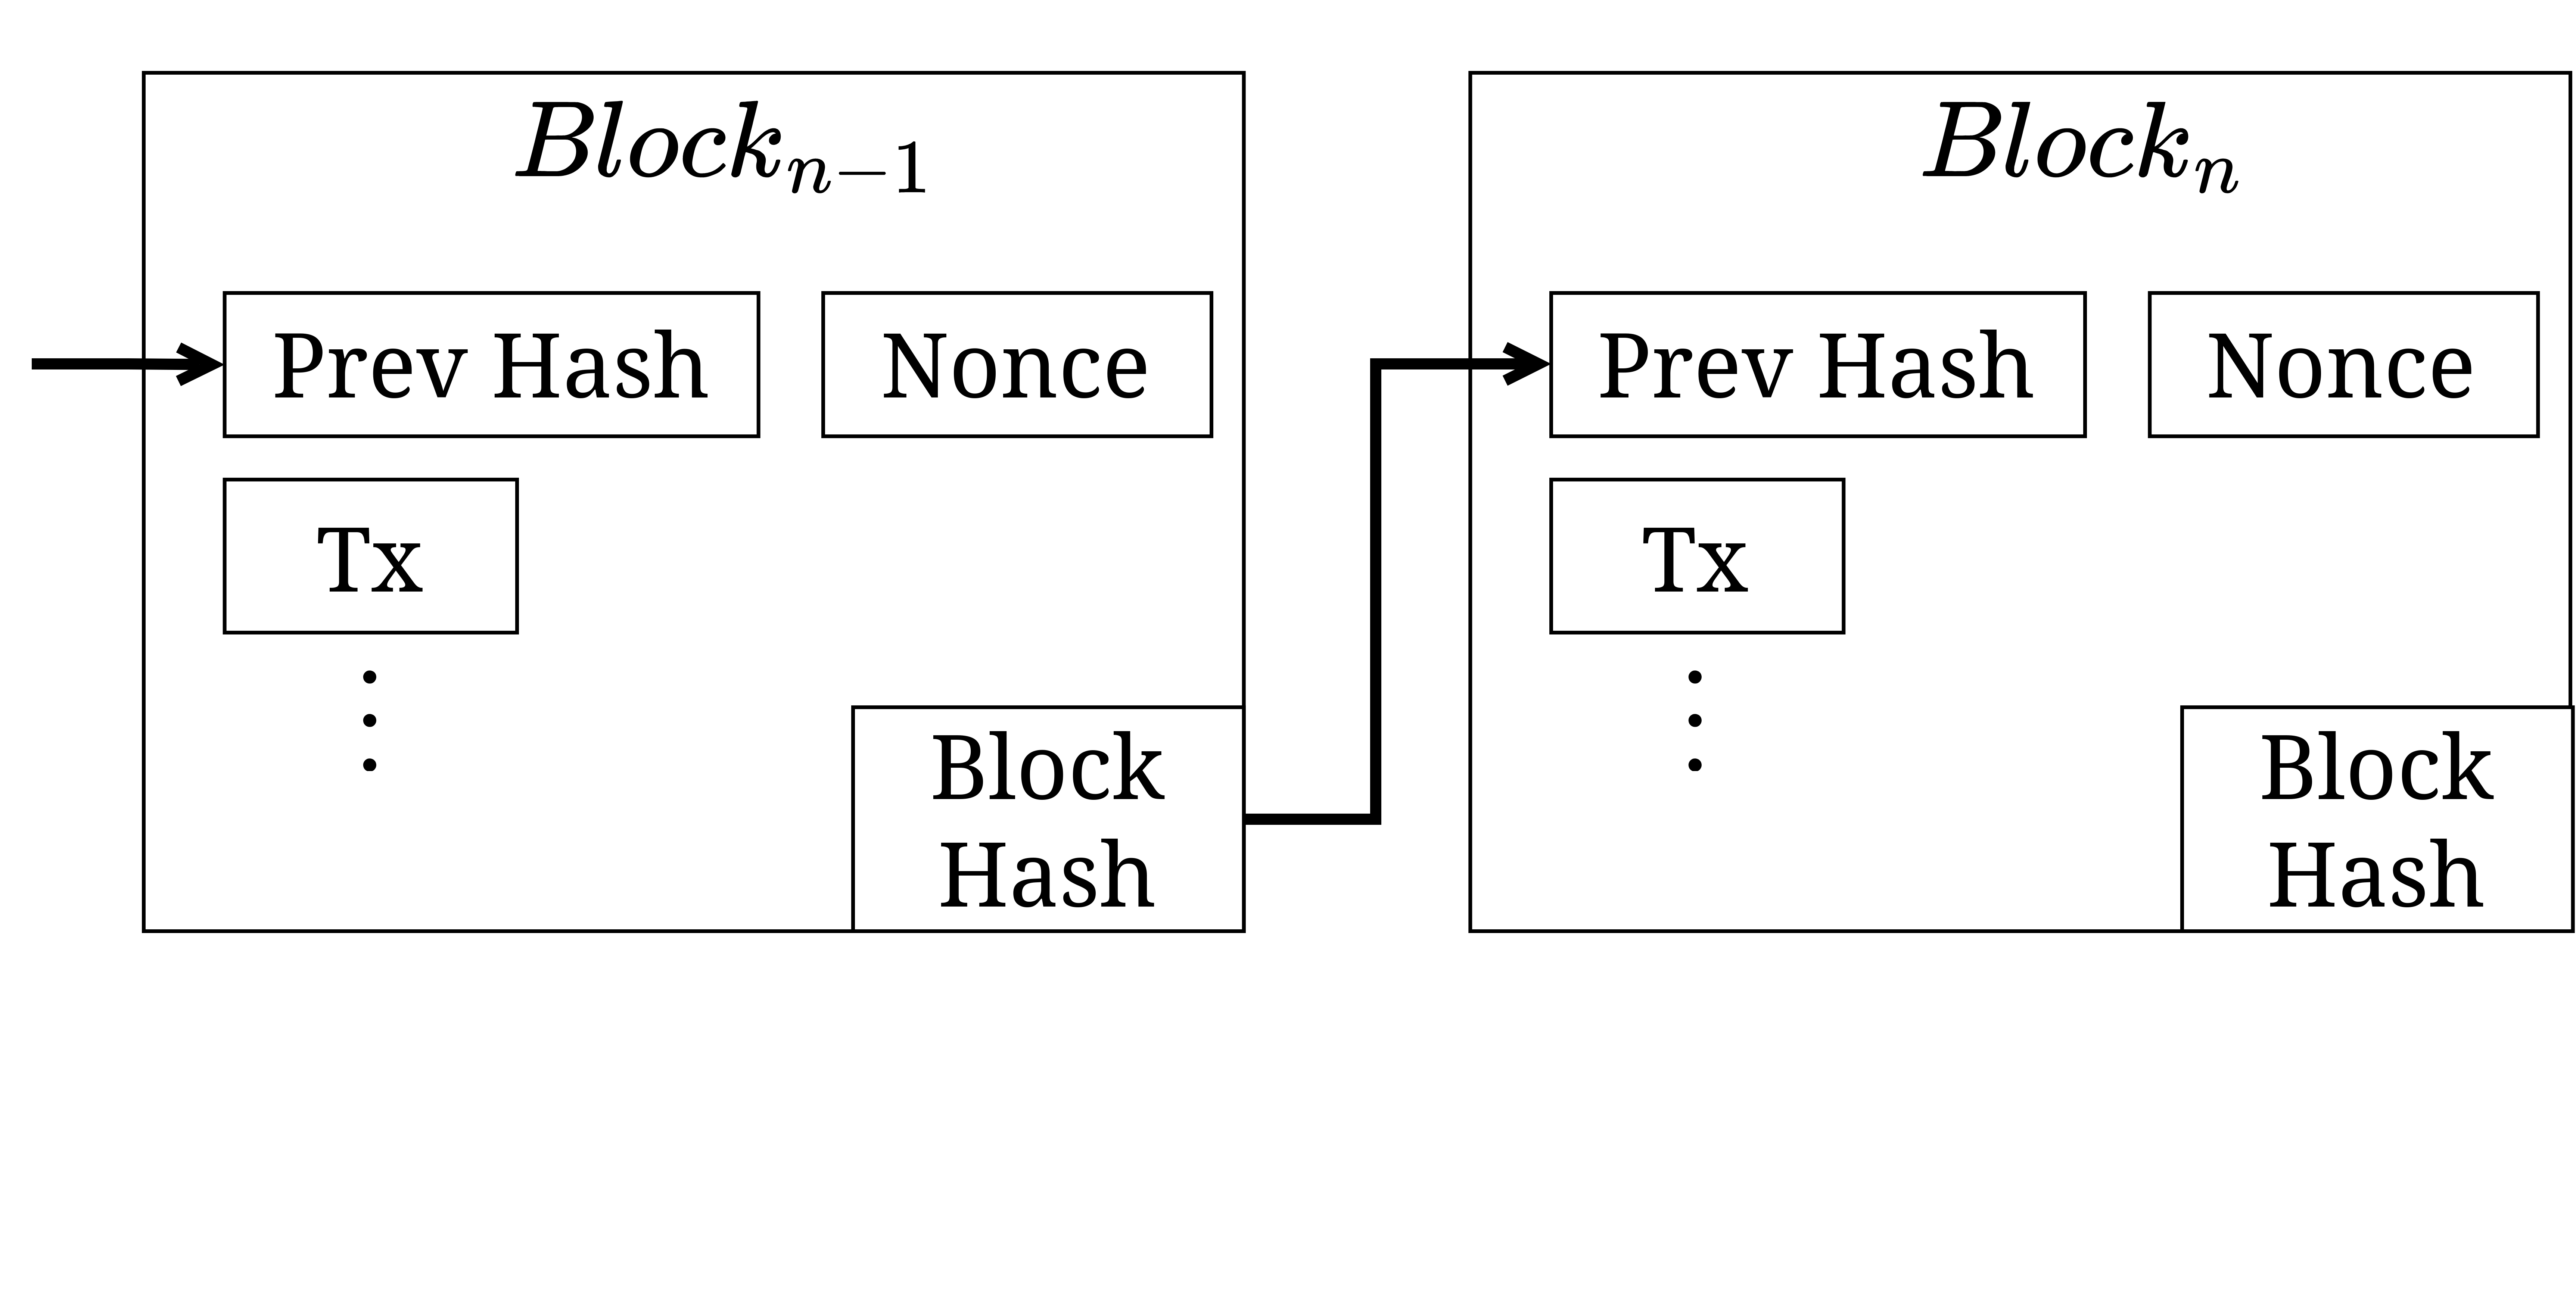
\includegraphics[width=\linewidth]{fig/blocks.png}
    \caption{A simplified overview of blocks, block hash is the output of the previous hash, the nonce value and the transactions (Tx) contained within that block.}
\end{figure}

This process requires a substantial amount of bandwidth and computing power, of course there must be 
an incentive to motivate the miners to keep mining (validating the network) and ensuring it operation, 
this incentive comes in the form of an extra transaction added to the mined block to be awarded for the
miner who successfully mines that block.

The fork choice mechanism: Longest chain rule, further reinforces PoW by providing a mean for resolving chain conflicts, if a node receives two contradicting versions of the chain with an equal
height from the genesis \footnote{The very first block published on the chain} that node only needs to wait for the chain that gets a newly mined block and considers
that chain to be the truth of the network, that is the chain with the most computational power spent to proof its validity through PoW.

There are significant downsides of both PoW and the longest chain rule: first PoW depends on draining scarce physical resources
in the form of electricity and mining hardware (GPUs, ASICs, etc.) in order to earn the mining reward. This model poses a grave
environmental threat \cite{btc:waste}, second the longest chain rule doesn't provide finality on a chain just the longest chain that exists,
and so an adversary can secretly work on an alternate chain, effectively removing transactions that were previously deemed valid and purpose
that alternative chain when it becomes longer than the original one.

\subsubsection{Proof-of-Stake}
Proof-of-Stake (PoS) an alternative consensus mechanism to PoW \cite{pos}, 
PoS replaces miners with validators, a validator gets the right to forge a new block
and that validator gets rewarded the transaction fees contained in that block.
In order to ensure that a validator would uphold the integrity of the network by not
approving fraudulent transactions, validators must first place stake in the network in 
the form of cryptocurrency that is higher than the transaction fees, if a validator approves
a fraudulent transaction they get penalized by getting part of their stake revoked.
The idea here is to have higher stake than the transaction fees so if a validator misbehaves
they'd lose more than they would gain from attempting to manipulate the network.
Validators get chosen to forge new blocks based on the amount of stake they've placed into
the network, the higher the stake the more likely it is a peer will become a validator of the next block.

\subsubsection{GHOST}
Greedy Heaviest-Observed Sub-Tree (GHOST) is an alternative fork choice algorithm \cite{ghost}, similar to Bitcoin's longest chain rule,
with one major difference is that it doesn't rely on the longest chain but rather choosing the chain associated with the most weight, rather
than just taking the longest one.

\begin{figure}[h]
    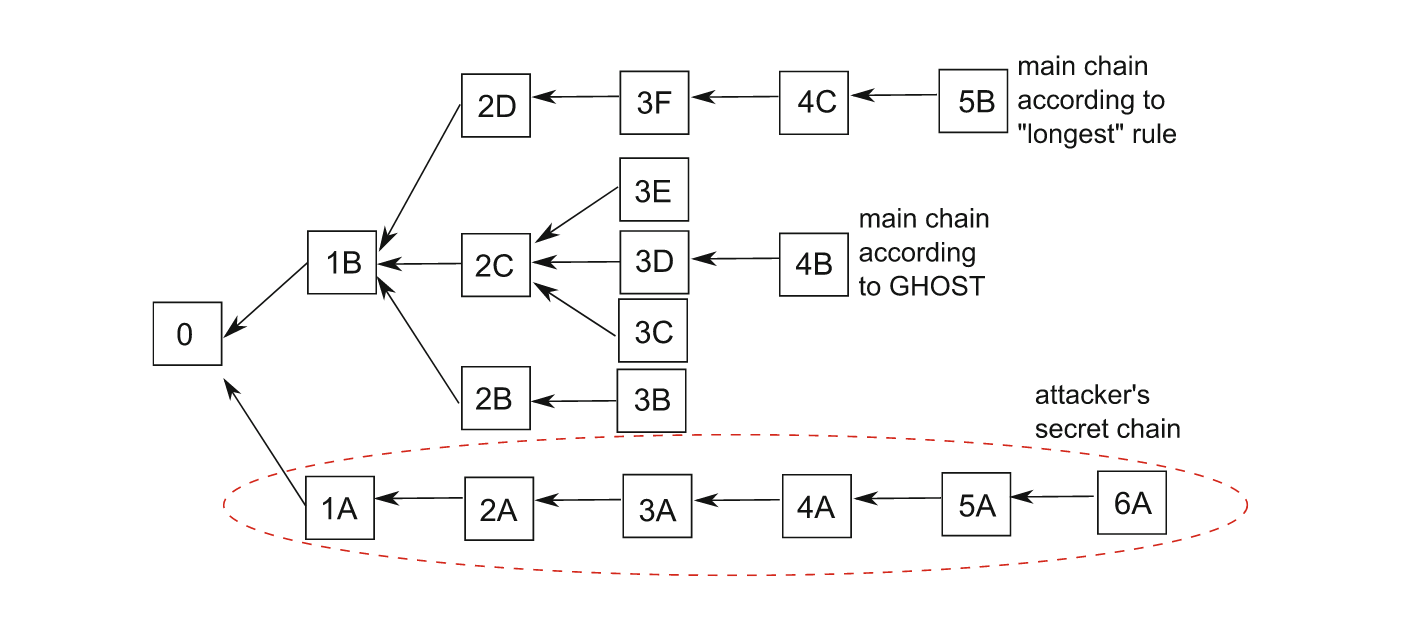
\includegraphics[width=\linewidth]{fig/ghost.png}
    \caption{\label{fork_attack}An attacker's chain is able to switch the longest chain, but not the chain selected by GHOST \cite{ghost}}
\end{figure}

\subsubsection{Casper FFG}
Casper the Friendly Finality Gadget (FFG) provides ``finality'' utility to blockchains. By finality, we mean
that the peers can come to consensus on blocks that are finalized and would never change, and these blocks
serve as \textbf{checkpoints} to the correct canonical chain, prior to that the only checkpoint a blockchain had is
its genesis block now it. Without checkpoints an attack can secretly fork a parallel chain to the canonical chain
and publish it when it satisfies the fork choice algorithm (See Figure \ref{fork_attack}).

Casper FFG puts blocks in three states:
\begin{enumerate}
    \item Proposed: The state at which a block has been proposed to the network
    \item Justified: In this state a block has been agreed upon via consensus and considered a part of the chain
    \item Finalized: In this state a block is changed into a checkpoint, so that it can no longer be revoked or modified.
\end{enumerate}

\section{Analysis}
In this section we give an overview of recent works and advancements in P2P security.

\subsection{GuardedGossip}
GuardedGossip is a proposed protocol for node discovery in Tor \cite{guarded_gossip}.
GuardedGossip builds on Chord DHT and enhances its security properties and defends against 
both active and passive attacks. In section \ref{DHT} we discussed that Chord is vulnerable to both passive attacks. 
A way to defend against passive attacks is via gossiping, by which nodes contact random nodes in the network, informing
them of their existance in the network as well as all the nodes that it knows off. This prevents information leakage. 
However, it's vulnerable to active attacks. GuardedGossip combines gossiping and DHT to build to grant immunity against
active attacks and significant reduce the possibility of passive attacks through uncertainty. 

In addition to chord standard shortcut table (\textbf{FT}), 
every node maintains extra information about the network summarized in the following:
\begin{itemize}
    \item Gossip List: contains nodes that sent us gossip requests.
    \item Witness List: contains nodes that we have ``seen'' during network operations along with a timestamp.
    \item Guarded List: contains nodes that are safe to establish connections with.
\end{itemize}

Now the protocol workflow goes as the following: a node is picked from the gossip list and added to the witness list,
then fetches the FT of the picked node and entries from that FT go through two checks:
\begin{enumerate}
    \item \textbf{Bound Checking}: compares the estimated average node density that is the difference between a finger entry and its corresponding optimal ID 
        (as if the entire chord ID space is occupied) we denote that density by $d$, the same process is applied to the fetched FT, again we denote it by $d_g$
        bound checking can then be expressed through the following constraint: $d_g < \gamma d$ where $\gamma$ is the \textit{finger table tolerance factor}.
    \item \textbf{Witness List Checking}: the witness list is used to detect malicious manipulation in the fetched FT whether some nodes were skipped.
\end{enumerate}

If any of the aforementioned checks failed the entire finger table is discarded; on the contrary if the fetched FT passed only a randomly
selected set of nodes are added to the guarded list generating uncertainty. Finally, the entirety of the passed FT is added
to the witness list to be utilized for future checks. Furthermore, the protocol maintains its lists by removing random entries
from both gossip and guarded lists generating even more uncertainty, and for the witness list entries are deleted based on their timestamp.

\begin{figure}
    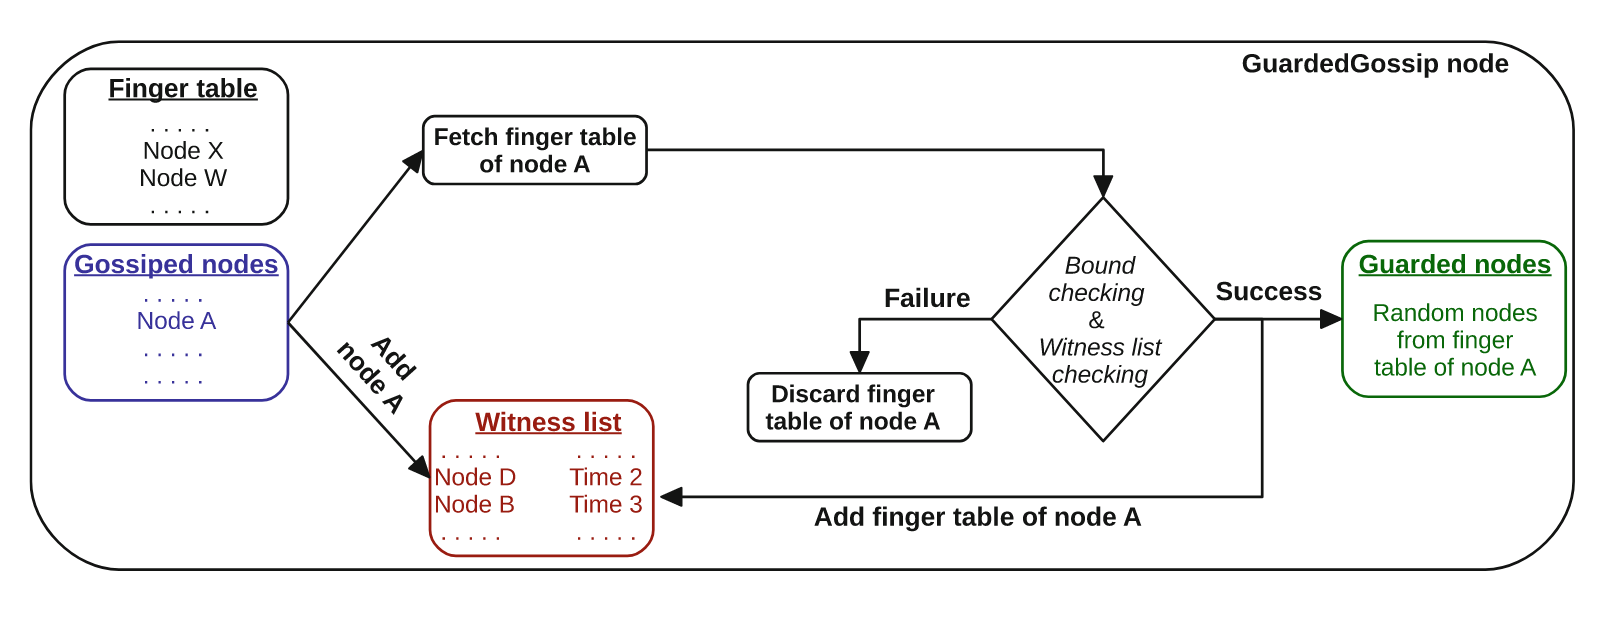
\includegraphics[width=\linewidth]{fig/guardedgossip.png}
    \caption{GuardedGossip protocol workflow \cite{guarded_gossip}}
\end{figure}

\subsection{GossipSub}
GossipSub is a message propagation protocol \cite{gossip_sub}, and is planned to be used in the Ethereum 2.0 Blockchain \cite{eth:network},
GossipSub combines ideas from Gossip and PubSub protocols to achieve efficient and secure message propagation, in section \ref{Blockchain} we discussed
the importance of publishing transactions and blocks to the network to maintain network security through consensus.

It does so by first constructing a mesh of local nodes, that is a partial view of the network. Whenever a new message is received it's immediately
forwarded to all nodes in the local mesh, as well as, sending meta-data about messages we have rather than the message itself to random nodes in
the network. Furthermore, each node keeps a score of its local mesh nodes via a scoring function, the score is not shared with other nodes in the network but rather
kept private. Now nodes can make more informed decisions on nodes to keep in its local mesh and nodes to prune from the mesh.
\begin{figure}[h]
    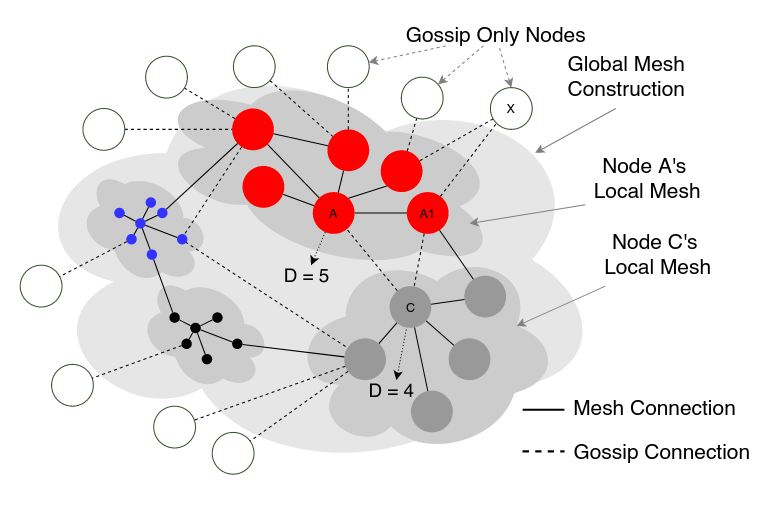
\includegraphics[width=\linewidth]{fig/gossip_sub.png}
    \caption{The GossipSub Mesh Construction \cite{gossip_sub}. $D$ refers 
    to the mesh degree (i.e., the number of nodes in the local mesh)
    }
\end{figure}

GossipSub provides an arsenal of defensive mitigation strategies to protect against the following attacks: Sybil, eclipse, censor, cold boot flash and covert flash.
\\
\\
\begin{enumerate}
    \item \textbf{Controlled Mesh Maintenance}: The local mesh hash two thresholds $D_{high}$ and $D_{low}$ 
        each node attempts to keep its mesh degree $D$ between these two thresholds by pruning (removing) or
        grafting (adding) nodes based on the score formed by the scoring function during network operation.

    \item \textbf{Opportunistic Grafting}: A node can get stuck in a mesh of bad performing peers and in this
        situation it might take a while before any new good performing peers are introduced, and so \emph{opportunistic
        grafting} mechanism checks the median score of current mesh and attempts to graft nodes that have score higher than
        median of the current mesh, this allows nodes with bad performing peers to quickly recover.

    \item \textbf{Flood Publishing}: newly published messages are sent to all known peers with a positive score that are
        subscribed to the topic.

    \item \textbf{Adaptive Gossip Dissemination}: a gossip factor is chosen to determine how many peers that are not part of the local mesh 
        receive gossip from the set of peers we know of the gossip factor was set to $25\%$ so that every node has a $50\%$
        chance of being picked during a gossiping round.
        This mechanism improve resistance against eclipse attacks.

    \item \textbf{Backoff on PRUNE}: Whenever a node is pruned in order to keep the mesh degree below $D_{high}$ it gets a \textit{backoff}
        during which it cannot send any GRAFT messages back to join that mesh again.
\end{enumerate}

\subsection{Saving Attack}
Ethereum 2.0 proposed two new fork choice rules \cite{eth2:spec} based on GHOST, fresh-message-driven (FMD) and latest-message-driven (LMD).
Gasper \cite{gasper} is a time-slot based PoS consensus mechanism that user Casper FFG \cite{casper_ffg} together with LMD GHOST to choose the
canonical chain of the network. Block proposal window is limited to a time \textbf{slot} every slot lasts for \textbf{12 seconds}
and every \textbf{32 slot} make up an \textbf{epoch}. Before an epoch starts individual peers are assigned as validators to each time slot and a committee of validators
is chosen to vote on the proposed block. The Saving Attack \cite{saving_attack} shows the possibility of malicious peers to delay the finality thus disrupting the network
and deviating the canonical chain from its current state to a modified state based on the blocks that had been ``saved'' by the attacker, \cite{saving_attack} shows that FMD GHOST
significantly reduces the impact of the saving attack.
\begin{figure}[h]
    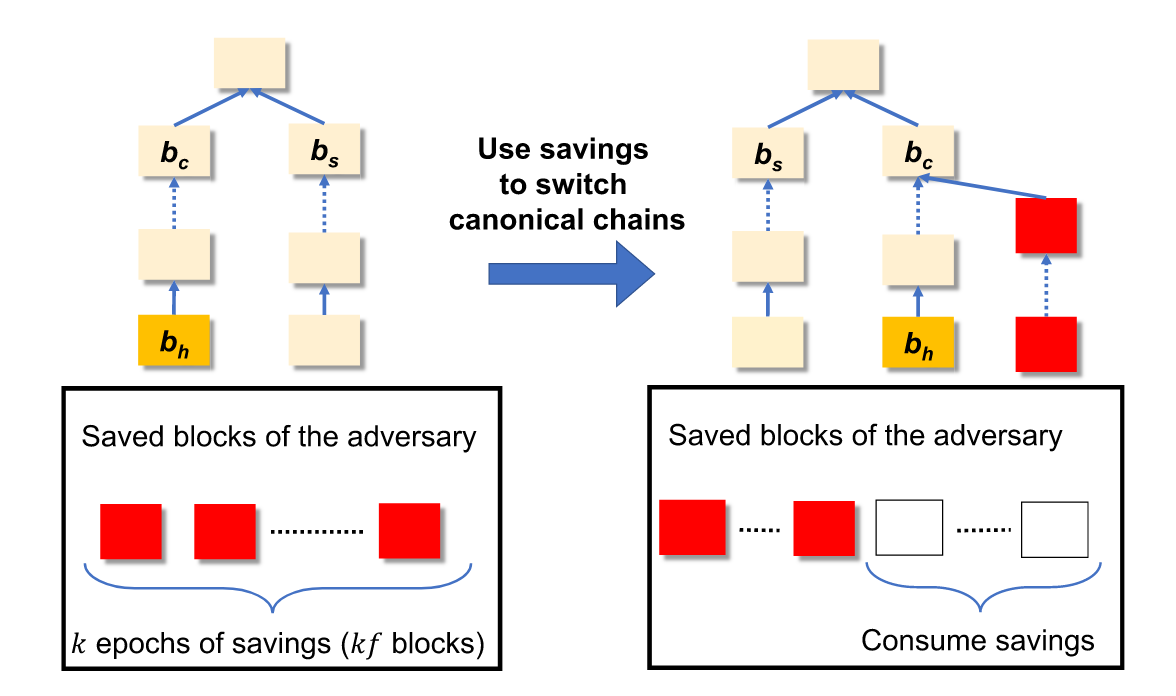
\includegraphics[width=\linewidth]{fig/saving_attack.png}
    \caption{Outline of the saving attack \cite{saving_attack}.
    $b_c$ denotes the canonical chain, $b_s$ denotes the secondary chain (that is the best candidate chain after the canonical one) 
    and $b_h$ denotes the current head block
    }
\end{figure}

\section{Evaluation}
In this section we present our results that we achieved while trying to replicate the simulation experiments performed in \cite{guarded_gossip},
the experiment was replicated with a major difference the network size. Although, our experiment network size is small we were able to achieve the same results,
which proves that GuardedGossip is applicable in small networks as well as being able to scale.
\begin{figure}[h]
    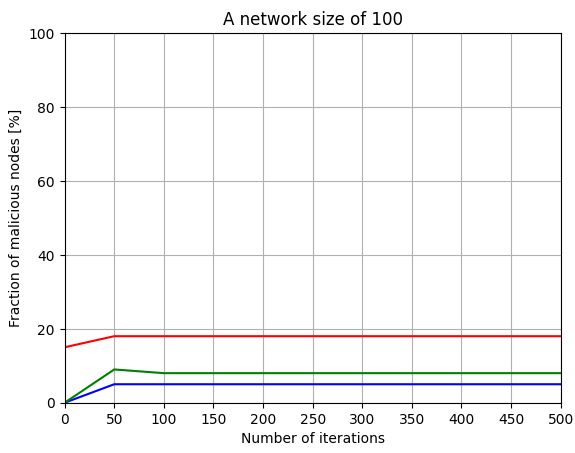
\includegraphics[width=\linewidth]{fig/experiment.png}
    \caption{\label{exper} Here we show that our results match the result from \cite{guarded_gossip} in a network of relatively low size.}
\end{figure}
\section{Conclusion and Future Work}
Pure P2P solutions are the way forwards, whenever we propose any form of hierarchy it automatically presents a target for attacks. The area of PoS based
blockchains is still new and the first major blockchain to widely adopt it is Ethereum which will attest to the security and performance of PoS for more 
blockchain applications to adopt, or perhaps we need a better consensus algorithm? One thing that is certain PoW is not sustainable and demands an urgent replacement.

On the other hand we can see the potential that a protocol such as GuardedGossip \cite{guarded_gossip} has in scaling Tor while preserving its security. However, it still has its flaws, 
as malicious peers can still find their into the guarded nodes list, extending the protocol with a scoring function like in \cite{gossip_sub} might have the potential to
significantly reduce the percentage of malicious nodes in the guarded list or perhaps even eliminate their existence in the network? We leave these questions for future works to further investigate.
\printbibliography
\end{document}
